% ****** Start of file apssamp.tex ******
%
%   This file is part of the APS files in the REVTeX 4.2 distribution.
%   Version 4.2a of REVTeX, December 2014
%
%   Copyright (c) 2014 The American Physical Society.
%
%   See the REVTeX 4 README file for restrictions and more information.
%
% TeX'ing this file requires that you have AMS-LaTeX 2.0 installed
% as well as the rest of the prerequisites for REVTeX 4.2
%
% See the REVTeX 4 README file
% It also requires running BibTeX. The commands are as follows:
%
%  1)  latex apssamp.tex
%  2)  bibtex apssamp
%  3)  latex apssamp.tex
%  4)  latex apssamp.tex
%
\documentclass[%
%reprint,
%superscriptaddress,
%groupedaddress,
%unsortedaddress,
%runinaddress,
%frontmatterverbose, 
preprint,
%preprintnumbers,
%nofootinbib,
%nobibnotes,
%bibnotes,
 amsmath,amssymb,
 aps,
%pra,
prb,
%rmp,
%prstab,
%prstper,
%floatfix,
]{revtex4-2}

\usepackage{graphicx}% Include figure files
\usepackage{dcolumn}% Align table columns on decimal point
\usepackage{bm}% bold math
\usepackage[inkscapeformat=png]{svg}
%\usepackage{hyperref}% add hypertext capabilities
%\usepackage[mathlines]{lineno}% Enable numbering of text and display math
%\linenumbers\relax % Commence numbering lines

%\usepackage[showframe,%Uncomment any one of the following lines to test 
%%scale=0.7, marginratio={1:1, 2:3}, ignoreall,% default settings
%%text={7in,10in},centering,
%%margin=1.5in,
%%total={6.5in,8.75in}, top=1.2in, left=0.9in, includefoot,
%%height=10in,a5paper,hmargin={3cm,0.8in},
%]{geometry}

\begin{document}

\preprint{APS/123-QED}

\title{Transition path sampling study of the MBHase reaction mechanism}% Force line breaks with \\
%\thanks{A footnote to the article title}%

\author{Sree Ganesh Balasubramani}
%\email{sreegb@arizona.edu}
% \altaffiliation[Also at ]{Department of Chemistry and Biochemistry, University of Arizona.}%Lines break automatically or can be forced with \\
\author{Steven Schwartz}%
 \email{sschwartz@arizona.edu}
\affiliation{Department of Chemistry and Biochemistry, University of Arizona.%
 }%

%\collaboration{MUSO Collaboration}%\noaffiliation

%\author{Charlie Author}
% \homepage{http://www.Second.institution.edu/~Charlie.Author}
%\affiliation{
% Second institution and/or address\\
% This line break forced% with \\
%}%
%\affiliation{
% Third institution, the second for Charlie Author
%}%
%\author{Delta Author}
%\affiliation{%
% Authors' institution and/or address\\
% This line break forced with \textbackslash\textbackslash
%}%

%\collaboration{CLEO Collaboration}%\noaffiliation

\date{\today}% It is always \today, today,
             %  but any date may be explicitly specified

%\begin{abstract}
%An article usually includes an abstract, a concise summary of the work
%covered at length in the main body of the article. 
%\begin{description}
%\item[Usage]
%Secondary publications and information retrieval purposes.
%\item[Structure]
%You may use the \texttt{description} environment to structure your abstract;
%use the optional argument of the \verb+\item+ command to give the category of each item. 
%\end{description}
%\end{abstract}

%\keywords{Suggested keywords}%Use showkeys class option if keyword
                              %display desired
\maketitle

%\tableofcontents

\section{\label{sec:level1}Introduction}
MBHase \cite{Crawshaw2022} 

\section{Transition path sampling}

\subsection{TPS ensemble}
The reaction well is defined through the 

\subsection{Committor analysis}

\begin{figure}[ht!]
\centering
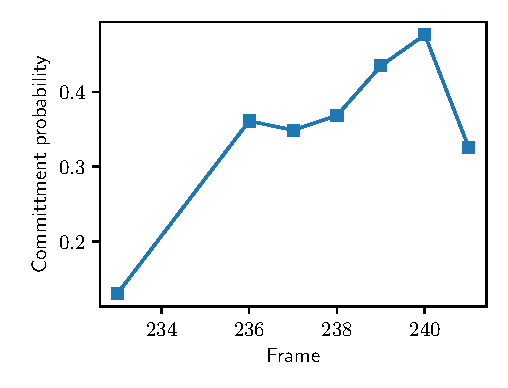
\includegraphics[scale=1.0]{figures/dist46.pdf}
\caption{The committor for several time frames}
\label{fig:comm-dist-46}
\end{figure}

\begin{figure}[ht!]
\centering
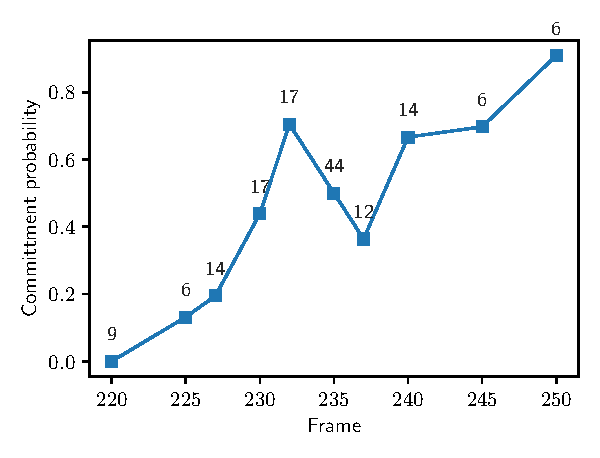
\includegraphics[scale=1.0]{figures/dist54.pdf}
\caption{The committor for several time frames for trajectory 54}
\label{fig:comm-dist-54}
\end{figure}

\bibliography{report}% Produces the bibliography via BibTeX.

\end{document}

